\section{Systementwurf} % Bitte sinnvolle Überschriften für alle Kapitel und Unterkapitel wählen
Der Abschnitt 'Systementwurf' beschreibt den umfassenden Entwurf des Collision Avoidance Assist-Systems. Das Ziel besteht darin, ein effektives und zuverlässiges System zu entwickeln, das in der Lage ist, potenzielle Kollisionen zu erkennen, den Fahrer zu warnen und bei Bedarf autonome Eingriffe zur Kollisionsvermeidung durchzuführen. Der Systementwurf umfasst die Spezifikation der Anforderungen, die Modellierung der Zustandsmaschine sowie die Definition der Schnittstellen mit anderen Komponenten. Durch eine gründliche Analyse und Planung wird ein robustes System geschaffen, das die Sicherheit und den Komfort des Fahrers verbessert. In diesem Abschnitt werden die einzelnen Aspekte des Systementwurfs detailliert beschrieben, um eine klare Roadmap für die Implementierung und den weiteren Entwicklungsprozess zu liefern.
\subsection{Spezifikation der Anforderungen}
Der Abschnitt 'Spezifikation der Anforderungen' beschreibt die grundlegenden Anforderungen an das Collision Avoidance Assist-System. Ziel ist es, ein System zu entwickeln, das potenzielle Kollisionsszenarien erkennt, den Fahrer rechtzeitig warnt und bei Bedarf autonome Eingriffe durchführt, um Kollisionen zu vermeiden. Das System soll verschiedene Sensoren wie Radar, Kamera oder LiDAR nutzen, um die Umgebung zu überwachen und Kollisionen in Echtzeit zu erkennen. Dieses Erkennungsmechanismus basiert auf die folgenden Aspekte:
\begin{itemize}
	\item Integration von Sensoren: Das System muss mehrere Sensoren, wie Radar, Kamera und LiDAR, integrieren, um Echtzeitdaten über die Umgebung zu sammeln.
	\item Objekterkennung: Das System muss in der Lage sein, Objekte, einschließlich Fahrzeugen, Fußgängern und Hindernissen, innerhalb eines bestimmten Bereichs, um das Fahrzeug zu erkennen und zu verfolgen.
	\item Bewertung des Kollisionsrisikos: Das System muss die Sensordaten analysieren, um das Kollisionsrisiko auf der Grundlage von Faktoren wie Objektabstand, Relativgeschwindigkeit und Flugbahn zu bewerten.
	\item Multi-Szenario-Erkennung: Das System muss in der Lage sein, potenzielle Kollisionsszenarien unter verschiedenen Fahrbedingungen zu erkennen, einschließlich gerader Straßen, Kurven, Kreuzungen und Parkplätzen.
	\item Verarbeitung in Echtzeit: Das System muss die Sensordaten verarbeiten und Entscheidungen zur Kollisionserkennung in Echtzeit treffen, um rechtzeitige Warnungen und Eingriffe zu gewährleisten.
\end{itemize}
%Die Spezifikation umfasst auch die Definition von Schnittstellen mit anderen Komponenten, um eine reibungslose Integration zu gewährleisten. In diesem Abschnitt werden die Anforderungen an die Kollisionserkennung, Warnungen und potenzielle autonome Eingriffe detailliert beschrieben, um eine klare Grundlage für den weiteren Entwurf und die Entwicklung des Systems zu schaffen.

\subsubsection{Art der potenziellen Kollisionen}
1. Fahrzeug-zu-Fahrzeug-Kollision (V2V):
\begin{itemize}
	\item Bei dieser Kollisionsart kollidieren zwei oder mehr Fahrzeuge miteinander.
	\item Das Kollisionsvermeidungssystem erkennt das Vorhandensein, die relative Position und die Geschwindigkeit von Fahrzeugen in der Nähe, gibt Warnungen aus und leitet möglicherweise Eingriffe ein, um die Kollision zu vermeiden oder zu entschärfen.
\end{itemize}
2. Kollisionen zwischen Fahrzeugen und Fußgängern (V2P):
\begin{itemize}
	\item V2P-Kollisionen treten auf, wenn ein Fahrzeug mit einem Fußgänger kollidiert, was ein erhebliches Risiko für die Sicherheit des Fußgängers darstellt.
	\item Das Kollisionsvermeidungssystem nutzt Sensoren und Algorithmen zur Erkennung von Fußgängern im oder in der Nähe des Fahrzeugs, gibt Warnungen aus und führt möglicherweise Brems- oder Lenkeingriffe durch, um die Kollision zu verhindern oder zu minimieren.
\end{itemize}
3. Kollisionen zwischen Fahrzeugen und Objekten (V2O):
\begin{itemize}
	\item Bei V2O-Kollisionen kollidiert ein Fahrzeug mit stehenden Objekten, wie z. B. geparkten Fahrzeugen, Leitplanken oder Hindernissen auf der Fahrbahn.
	\item Das Kollisionsvermeidungssystem erkennt die Anwesenheit und Nähe von Objekten, gibt Warnungen aus und leitet möglicherweise Brems- oder Lenkeingriffe ein, um die Auswirkungen der Kollision zu vermeiden oder zu verringern.
\end{itemize}
4. Kollision zwischen Fahrzeug und Radfahrer (V2C):
\begin{itemize}
	\item V2C-Kollisionen treten auf, wenn ein Fahrzeug mit einem Radfahrer kollidiert, der die Straße mit Kraftfahrzeugen teilt.
	\item Das Kollisionsvermeidungssystem kann die Anwesenheit von Radfahrern erkennen, ihre Bewegungen vorhersagen und Warnungen ausgeben oder Eingriffe einführen, um Kollisionen zu verhindern oder abzuschwächen.
\end{itemize}
5. Auffahrunfall:
\begin{itemize}
	\item Zu einem Auffahrunfall kommt es, wenn ein Fahrzeug auf das vorausfahrende Fahrzeug auffährt, weil der Abstand nicht ausreicht oder zu spät gebremst wird.
	\item Das Kollisionsvermeidungssystem kann die relative Geschwindigkeit und den Abstand zwischen den Fahrzeugen überwachen, Warnungen ausgeben und möglicherweise automatisch bremsen, um Auffahrunfälle zu vermeiden oder zu minimieren.
\end{itemize}
6. Seitenkollision:
\begin{itemize}
	\item Zu einer Seitenkollision, auch T-Bone-Kollision genannt, kommt es, wenn ein Fahrzeug von einem anderen Fahrzeug seitlich getroffen wird.
	\item Nur ein kleiner Anteil mancher Kollisionsvermeidungssysteme verwenden Sensoren und Algorithmen, um das Risiko von Seitenkollisionen zu erkennen und Warnungen oder Eingriffe vorzunehmen, um die Schaden solcher Kollisionen zu verringern.
\end{itemize}
7. Frontalzusammenstoß:
\begin{itemize}
	\item Bei einem Frontalzusammenstoß (auch Head-On Collision genannt) stoßen zwei Fahrzeuge zusammen, die in entgegengesetzter Richtung fahren, was oft zu schweren Schäden und Verletzungen führt.
	\item Während sich Kollisionsvermeidungssysteme in erster Linie auf vorwärts gerichtete Szenarien konzentrieren, können sie Sensordaten und Vorhersagealgorithmen nutzen, um das Risiko von Frontalkollisionen zu erkennen und Warnungen oder Eingriffe vorzunehmen, um diese zu verhindern oder abzuschwächen.
\end{itemize}

\subsubsection{Art und Weise der Warnungen}


%\begin{figure}[H]
%	\centering	
%	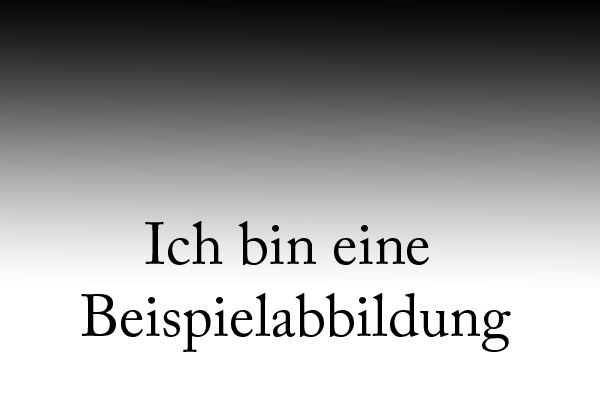
\includegraphics[width=.5\textwidth]{img/sample}
%	\caption[Beispielabbildung]{Beispielabbildung}
%	\captionsource{So könnte man z.b. die Bildquelle angeben}
%	\label{fig:Sample}
%\end{figure}
\subsection{Unterabschnitt 2}

\subsection{Unterabschnitt 3}

\subsection{Unterabschnitt 4}


\section{Hauptteil 2}
